\section{Architecture}

This section covers the architecture of the developed library, primary components and modules, the sequence of operations processing on the GPUs. The library is designed in order to overcome the limitation of the existing solutions, mentioned in the previous section.

\subsection{Design principles}

SPLA library is designed the way to maximize potential library performance, simplify its implementation and extensions, and to provided the end-user verbose, but effective interface allowing customization and precise control over operations execution. These ideas are captured in the following principles.

\begin{itemize}
    \item \textbf{OpenCL API}. The library must use the OpenCL API to accelerate computations on a single OpenCL-compatible GPU device in the system. This API is supported on a variety of graphics accelerators, and also allows you to dynamically compile GPU code at runtime, which saves the user from installing and using a third-party specialized compiler.

    \item \textbf{DAG-based expressions}. The user defines tasks for computations in the form of a directed acyclic graph of expressions, using the library interface to create graph nodes and dependencies between nodes in a declarative style. The user then passes the entire graph to the library for execution, and can either block or wait in a non-blocking way the result.
    
    \item \textbf{User data types}. The library provides the ability to create arbitrary custom types. The type is represented by the unique name and size of the elements in bytes. The elements of the type are POD structures, treated as regular byte sequences.
    
    \item \textbf{User functions}. The library provides the ability to create user-defined functions that can take user-defined (arbitrary) types as input, and which can be used to parameterize mathematical operations. Functions are defined as a set of sinks with OpenCL code, which allows you to create functions without using third-party tools to compile custom code.
    
    \item \textbf{Automated scheduling}. The library automatically splits the expression graph into many tasks and subtasks, which are ordered according to dependencies and distributed to the GPU device. This work is hidden from the user and does not require any action from him.
    
    \item \textbf{Automated hybrid storage format}. The library automatically formats the data, stores it in a hybrid format, and distributes it automatically between the computing device and the host. This work, storage format, distribution details are hidden from the user and do not require any action from him.
    
    \item \textbf{Exportable interface}. The library has a C++ interface with an automated reference-counting and with no-templates usage. It can be wrapped by C99 compatible API and exported to other languages, for example, in a form of a Python package.
\end{itemize}

\subsection{Execution}

The general idea of the library expression execution is depicted in the figure~\ref{fig:execution_schema}.

As an input library accepts the expression in a form of DAG. The DAG is created using library API. Vertices of the computational graph are the fundamental operations, which process primitives such as matrices or vectors. This operations can read or write data, compute product, etc. Directed edges between vertices show data dependencies between operations. If the edge is present between operations, then the next operation is executed only after the previous one is fully finished. This approach allows to specify, which operations must be ordered and which one can be executed in parallel, what allows better occupy the GPU device.

\begin{figure}[ht]
    \centering
    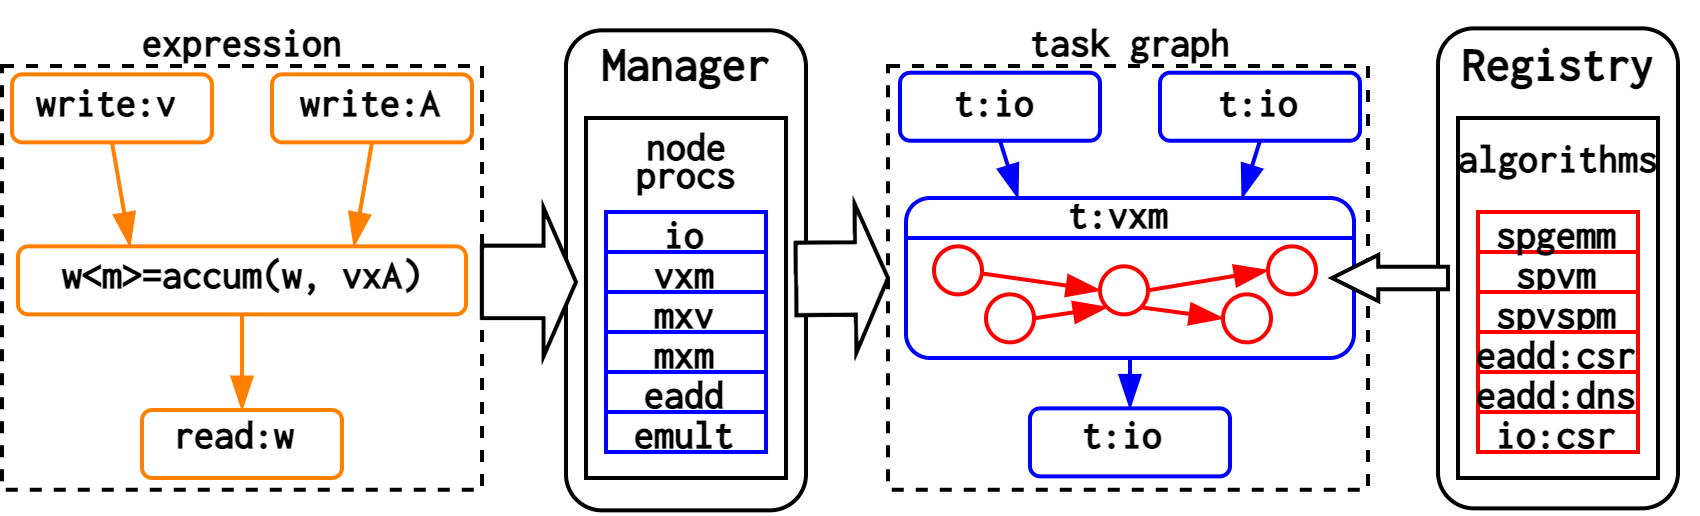
\includegraphics[width=1.0\textwidth]{images/execution_schema.png}
    \caption{Library expression processing schema.}
    \label{fig:execution_schema}
\end{figure}

The DAG expression is submitted to the library for the execution. The expression is traversed and for each a specialized processor is found. The processor is responsible for a processing of a single node. It is possible to have multiple processors for a single type operations with specialized rules of selection. This approach allows to separate the data and the execution, as well as gives an ability to handle some edge cases and optimize operation for a particular set of input arguments.

Processors are used to construct a task graph from the expression. Each processor adds tasks and subtasks for the execution of a particular node. External dependencies between nodes are preserved and translated into dependencies between tasks. Dependencies between subtasks inside a single task are defined by a node processor. 

Subtasks are spawned regardless of the storage format and parameters of a particular input arguments. For each type of the arguments there may be present a specialized algorithm in the registry. Algorithm is selected automatically at runtime using a set of rules and priorities. It is possible to specialize algorithm for any type of format and register them without processor code modification. 

The task graph is scheduled a whole object to the execution on a multi-core GPU in a multi-threaded mode. CPU threads process tasks and subtasts in a safe manner, since all data dependencies are preserved due to the nature of submitted DAG expression. Each subtask uses separate GPU scheduling queue, so it offloads the GPU with a work without serialization.

Expressions are executed asynchronously. The user after submission gets a special \textit{future} object, which allows either to block until completion or to probe the state of the expression in a non-blocking fashion.

\subsection{Storage}


